%!TEX root = ../thesis_phd.tex
%%%%%%%%%%%%%%%%%%%%%%%%%%%%%%%%%%%%%%%%%%%%%%%%%%%%%%%%%%%%%%%%%%%%%%%%%%%%%%%%
%neutrino_physics.tex: Chapter on neutrino physics:
%%%%%%%%%%%%%%%%%%%%%%%%%%%%%%%%%%%%%%%%%%%%%%%%%%%%%%%%%%%%%%%%%%%%%%%%%%%%%%%%
\chapter{Neural Networks}
\label{nnet_chapter}
%%%%%%%%%%%%%%%%%%%%%%%%%%%%%%%%%%%%%%%%%%%%%%%%%%%%%%%%%%%%%%%%%%%%%%%%%%%%%%%%

% test line

The field of machine learning is concerned with algorithms which can learn to make predictions from data.  Typically this involves some form of multivariate function approximation.  In other words, given some set of input variables, predict some set of output variables.  If the goal is to predict one or more outputs of a continuous function, the task is referred to as regression.  The task of separating examples into groups is called classification.

It is also common to separate machine learning approaches into two categories: supervised and unsupervised.  The supervised approach involves training an algorithm using a collection of examples for which the function output is known.  In unsupervised learning, algorithms can work to extract meaningful output from data where the function output is not known.

The approach presented in this thesis applies a supervised learning strategy for both classification of signal events and regression to approximate the energy of those events.



\section{Artificial Neural Networks}

An artificial neural network is a common tool used in classification and regression.  This class of algorithms draws inspiration from biological neurons.  Nervous systems of organisms are built up from a repeated structure of cells, called \textit{neurons}, which are connected to each other in order to transmit signals.  An example of a neuron can be seen in figure \ref{neuron}.  The base of a neuron is formed by a branching tree of \textit{dendrites} which receive signals from other neurons.  Signals are integrated and amplified in the cell body, then retransmitted through a long shaft, or \textit{axon}, to other neurons.  Intelligence is achieved by connecting many neurons which produce a wide variety of responses based on given stimuli.


\begin{figure}[t]
  \begin{center}
    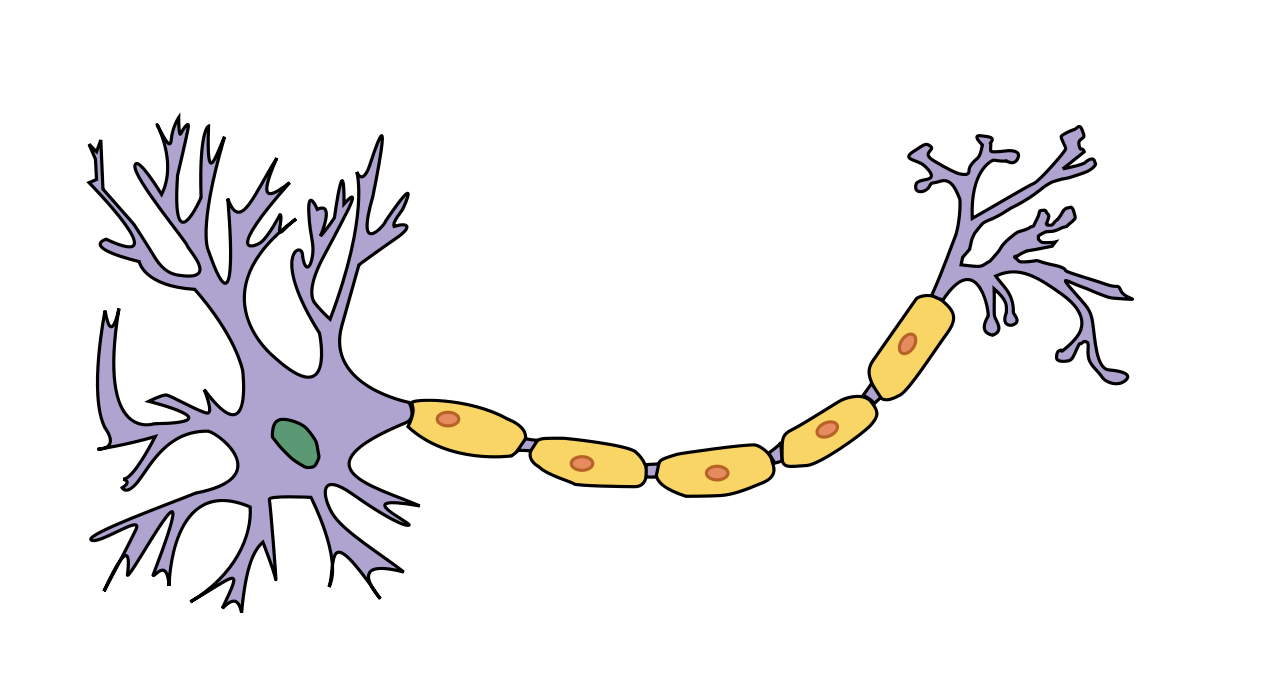
\includegraphics[width=0.7\textwidth]{figures/figures/neuron.png}
  \end{center}
  \caption[A basic rendering of a biological neuron]{A basic rendering of a biological neuron.  Signals are received through the branching dendrites to the left of the image.  The cell body integrates and retransmits signals to other cells through the axon, which runs horizontally from left to right in the figure.  Biological nervous systems are based upon a repeated structure of neurons to carry signals over long distances.}

  \label{neuron}
\end{figure}

Artificial neural networks are designed to crudely approximate the structure of a biological nervous system \cite{reed1999neural}.  The basic unit of a neural network is called a \textit{node}.  Each is a function which computes an output value from a set of inputs.  Nodes are arranged into \textit{layers}, as seen in figure \ref{nnet}.  In graph theory terms, a neural network is a \textit{feedforward graph}, implying that information is passed forward to subsequent layers, but not backward.  Input variables to the classification or regression problem are passed through \textit{input layer}, and the .  Any number of downstream \textit{hidden layers} can be trained to perfrom the classification or regression task.  The predicted output is then extracted from the final \textit{output layer}.  For multivariate regression, the output is a vector of decimal values.  For multi-class classification, the output is ususally a vector of as many values as there are classes, each ranging between zero and one.  The  magnitude of the each value is interpreted as how well the inputs represent that particular class.

Each node in a layer typically receives input from all nodes in the previous layer, although more sparesely connected networks have been investigated.  The response to each input is characterized by a set of weights, $\mathbf{w}^{i,j}$, for node $i$ in layer $j$.  Each layer produces a vector of outputs, $\mathbf{a}^{j}$, so the response in for the $i$th node in layer $j$ is the inner product between the weight vector of the node and the outputs of the previous layer in addition to a bias term, $b^{i,j}$:

\begin{equation}
z^{i,j} = \mathbf{w}^{i,j} \circ \mathbf{a}^{j-1} + b^{i,j}
\end{equation}

The node response is commonly passed through some nonlinearity, $f(x)$ to produce the output to be passed to the next layer, thus the element in $\mathbf{a}^{j}$ for the $i$th node is:

\begin{equation}
a^{i, j} = f(z^{i,j})
\end{equation}

Common choices for the nonlinearities are the sigmoid function, hyperbolic tangent ($\tanh$),rectified linear unit (\relu) or softmax.
\begin{align}
f(x) &= \frac{1}{1+e^x}  \tag{Sigmoid}\\
f(x) &= \frac{e^x-e^{-x}}{e^x+e^{-x}} \tag{$\tanh$} \\
f(x) &= \max(0,x) \tag{\relu}  \\
f(x) &= \frac{e^{x_i}}{\sum_{k} e^{x_k}} \tag{Softmax}  \\
\end{align}
The index in softmax enumerates the outputs of the other nodes in the same layer.
The softmax is thus normalized such that the sum of outputs from that layer is equal to one.
This feature makes the softmax a popular choice for output nodes in classification tasks since it provides a convenient pseudo-probabilistic interpretation of the output values.

Sigmoid and $\tanh$ are attractive because they are bounded, differentiable.  Rectified linear units are more analogous to the thresholded linear response of a biological neuron.  The negative component of range of the $\tanh$ is thus poorly motivated based on biological neurons, which do not produce a negative response.
Even still, tanh nonlinearities have been observed to produce good results.
\relu is additionally attractive since it does not involve the exponential function, which is expensive to evaluate from a computational standpoint.
Meanwhile, the unbounded derivative of \relu can lead to problems during gradient-based training, discussed in section \label{backprop}.
This trouble is commonly averted bu imposing an artificial bound on the derivative of the \relu.
It should also be noted that while the \relu is not differentiable at zero, it is differentiable arbitrarily close to zero, which is sufficient for training.

The input layer to the neural network depends on the problem at hand.  Basic applications of neural networks involve some number of input variables ranging from a few to a few hundred.  In some cases, the inputs are a set of engineered features extracted from some raw data, while other cases input raw data directly into a network.  The capacity for a network to learn to solve a particular problem increases with the number of hidden layers.  For practial reasons which will be discussed in section \ref{deeplearning}, diminishng returns are typically seen with more than a few hidden layers unless special techniques are applied.


\begin{figure}[t]
  \begin{center}
    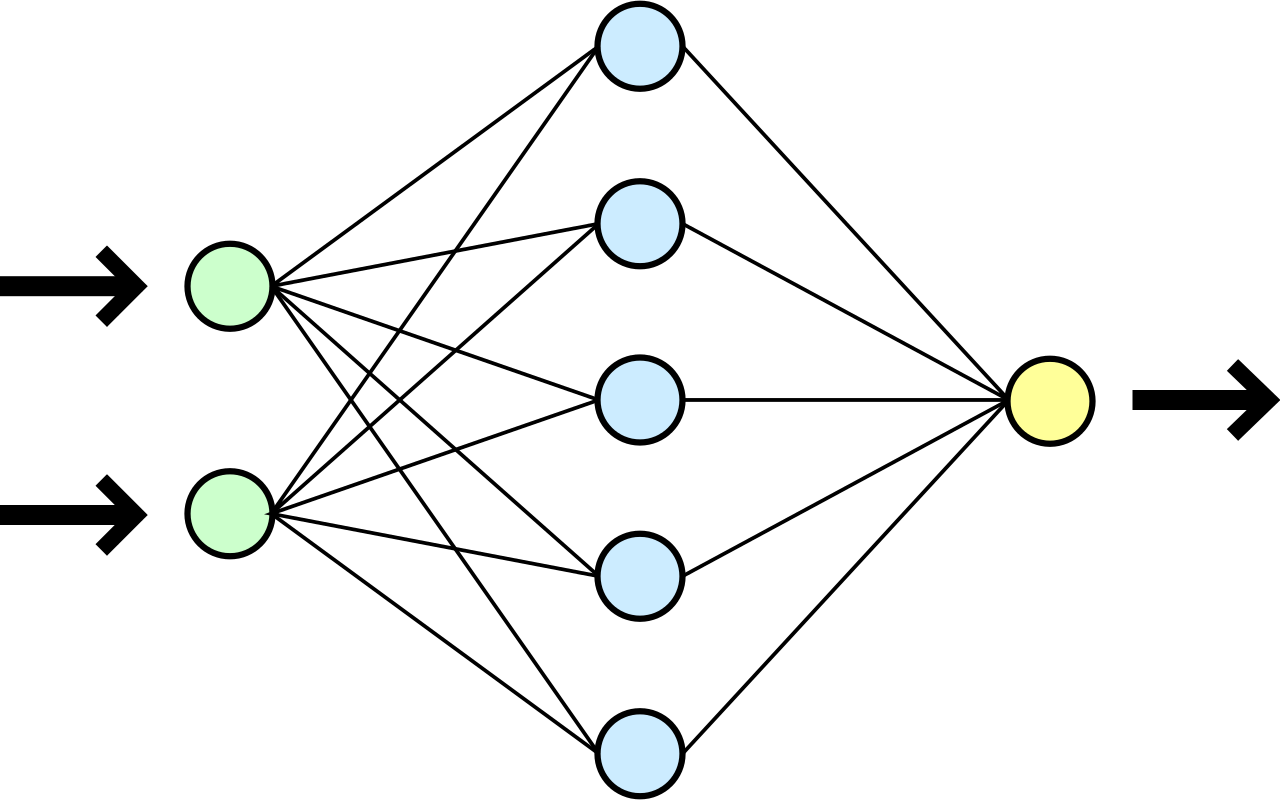
\includegraphics[width=0.5\textwidth]{figures/figures/basicNN.png}
  \end{center}
  \caption[Visualization of a simple neural network ]{Visualization of a simple neural network.  This network has an input layer (green) with two nodes, a hidden layer (blue) with five nodes, and an output layer (yellow) with one node.}

  \label{nnet}
\end{figure}


\section{Supervised Learning -- Backpropagation}
\label{backprop}

While neural networks were first proposed in the 1950s, practical applications were out of reach until a supervised learning strategy called backpropagation was introduced by Werbos in 1974 \cite{werbos1974beyond}.  Backpropagation is a supervised learning algorithm; the network is presented with a set of training examples with a known output as an iterative process to learn optimal weight parameters.  The major step forward in the backpropagation is a clever application of the chain rule to differentiable nonlinearities, thus allowing steepest descent stochastic gradient descent (SGD) to be used for training.

SGD is a common optimization technique.  If there is some objective function to be optimized, SGD seeks optimal parameters using the gradient that function.  Over many iterations, a function can be approximately minimized by adjusting the parameters opposite the gradient of the objective function at a given iteration step.  This gives the update rule for the weights $w$
\begin{equation}
w \coloneqq w - \eta \nabla E(w).
\end{equation}
The parameter $\eta$ is referred to as the \textit{learning rate}, which governs the step size.  Generally, $\eta$ is set to some value between 0 and 1, although there is no straightforward way to determine a value which will give the quickest or optimal convergence.  Large values for the learning rate may speed up convergence, but might also cause the algorithm to repeatedly step over the minimum location in the surface given by the objective function.

There are many variants of SGD which are popular.  Backpropagation itself does not specify which variant of SGD should be applied, it merely provides a mechanism to calculate the partial derivative with respect to each weight parameter.  At the core of backpropagation is a simple, but clever, application of the chain rule to find the derivative at an arbitrary node upstream of the output in a feedforward network.

First, the predicted output is calculated for a set of training examples are calculated in a feedforward pass.  An objective function is chosen to quantify the error between the target and predicted outputs.  Minimizing the objective function through an iterative process thus trains the network to predict the target outputs.  In regression problems, the objective function is commonly some mean-square error on the Euclidean distance between the target outputs and predicted outputs.  A simple implementation, for a network with outputs $m$ and training examples $p$ is
\begin{equation} E = \frac12 \sum_p \sum_m (t_{mp} - y_{mp})^2
\label{rmse}
\end{equation}
where $t_{mp}$ and $y_{mp}$ respectively correspond to the target and predicted output of the network.  The factor of $\frac12$ is simply present for cancellation after taking the derivative.  Classification problems commonly use another form of the objective function called the cross-entropy.  For output classes $m$, and again training examples $p$, target $t$ and prediction $y$, the cross entropy is:
\begin{equation}
E = \sum_p \sum_m t_{mp} \ln(y_{mp}) + (1-t_{mp})\ln(1-y_{mp})
\end{equation}

Backpropagation can be applied to any feedforward network of nodes with differentiable nonlinearities.  A layered structure is not a required.  Therefore, the process can be described by idexing $w_{ij}$ as the weight \textit{from} node $j$ to node $i$.  A feedforward network implies $j>i$ is not allowed.  The forward pass thus defines the inner product for each node, $a_i$, as a function of the weights and upstream nodes
\begin{equation}
a_i = \sum_{j<i} w_{ij} y_j.
\end{equation}
Above, $y_i$ is the result of the nonlinearity for each node
\begin{equation}
y_i = f(a_i).
\end{equation}

Backpropagation finds a partial derivative for each weight by summing over a batch of training examples.  The overall partial derivatives for the weight to node $i$ from weight $j$ is the sum of the gradients from training examples $p$:
\begin{equation}
\frac{\partial E}{\partial w_{ij}} = \sum_p \frac{\partial E_p}{\partial w_{ij}}
\end{equation}
The partial derivative for a particular training example can be written in terms of the upstream node outputs $a_k$
\begin{equation}
\frac{\partial E_p}{\partial w_{ij}} =
\sum_k \frac{\partial E_p}{\partial a_k} \frac{\partial a_k}{\partial w_{ij}} =
\sum_k \delta_{kp} \frac{\partial a_k}{\partial w_{ij}},
\end{equation}
with $\delta_{kp}$ defined for convenience:
\begin{equation}
\delta_{kp} = \frac{\partial E_p}{\partial a_{kp}} = \frac{\partial E_p}{\partial y_{kp}}\frac{\partial y_{kp}}{a_{kp}}.
\end{equation}
The second term is just the derivative of the nonlinearity, $f$
\begin{equation}
\frac{\partial y_{kp}}{a_{kp}} = f'(a_{kp}).
\end{equation}

The output nodes have no dependence on upstream nodes.  For the mean-square error mean-square objective function, for instance, we have:
\begin{equation}
\delta_{kp} = -(t_{pk} - y_{pk})f'(a_{kp}).
\end{equation}
The partial derivative of the cross-entropy objective, on the other hand, is:
\begin{equation}
\delta_{kp} = \bigg(\frac{t_{pk}}{y_{pk}}- \frac{1-t_{pk}}{1-y_{pk}}\bigg)f'(a_{kp}).
\end{equation}

The derivative of the objective function with respect to the weights in the hidden layers depends on downstream layers, so the chain rule must be applied.  The derivative for the $k$th hidden node relative to the $p$th training example is
\begin{equation}
\delta_{kp} = \frac{\partial E_p}{\partial a_{kp}} = \sum_l \frac{\partial E_p}{\partial a_{lp}}\frac{\partial y_{lp}}{a_{kp}}.
\end{equation}
The first factor in the sum is simply $\delta_{lp}$.  The second factor is zero if node $k$ does not connect to node $l$, otherwise it simply the product of the node connection weight and the slope of the nonlinearity for that node, evaluated for that training sample:
\begin{equation}
\frac{\partial a_{lp}}{a_{kp}} = f'_{lp} w_{lk}
\end{equation}
Thus, for hidden nodes, we have:
\begin{equation}
\delta_{kp} = f'_{kp} \sum_l w_{lk}\delta_{lp}
\end{equation}

Backpropagation drove a major shift in the field of neural networks.  Prior to the innovation of backpropagation, researchers focused their time on the theoretical capacity of networks of binary hidden units.  Armed with backpropagation, research could be devoted to applications, but now using differentiable hidden units trained with SGD.


\section{Deep Learning}
\label{deeplearning}

From a theoretical perspective, deep neural networks -- those with many layers -- offer increased capacity for problem solving by forming higher order nonlinear functions.  There are technical difficulties involved in the training of deeper networks, however.  The increase in complexity for larger networks can lead to serious constraints around the requisite computing power.  Further, backpropagated derivatives can become small in upstream layers, causing very little learning to occur in those layers.  For decades, these constraints required applications to be developed around a small set of features extracted from raw data rather then the raw data itself.  Engineering of those features is commonly a meticulous process involving considerable domain knowledge.  Recent innovations in network architecture and training strategy have led to major advances in performance, particularly in the field of computer vision and recognition.
Applications of neural networks now commonly involve deep architectures with many inputs.
In the case of image processing problems, it is not uncommon to use upwards of several thousand raw pixels as input and tens of hidden layers \cite{lecun2015deep}.
This section is not a complete survey of techniques used in deep learning, which are many, but merely a description of the techniques used in this thesis.

\subsection{Convolution Layers}

Use of convolution layers has led to top results in the field of computer vision \cite{lecun2010convolutional,krizhevsky2012imagenet}.  These layers are inspired by studies of the visual cortex of animals  \cite{lecun2015deep}, in which groupings of neurons scan over small sub-regions of the visual field.  Independent treatment of sub-regions can allow the networks at large to detect learned features in a position-independent fashion.  In other words, classification of an image can be achieved even if the subject appears in a different location within the frame.  In an artificial neural network, this is achieved using a  discrete convolution operation.  The convolution of discrete sequences $f$ and $g$ is defined as
\begin{equation}
(f*g)_i = \sum_{j = -\infty}^{\infty} f_j g_{i-j}.
\end{equation}
For convolution layers, the sequence $g$ to be the image and $f$ is called a filter.  Instead of ranging from $-\inf$ to $\inf$, the filter is restricted to have non-zero values over a finite range corresponding to an $n \times n$ pixel sub-region of the image.  The square sub-region of the image is ``unrolled'' into a one dimensional vector in order to support the convolution.  The filter weights, $f_j$, are can be learned through backpropagation to learn features within the image.  The output of a convolution layer has each pixel replaced with the output of $f$ convolved over the surrounding $n\times n$ sub-region.  A convolution layer can have many such filters, leading to multiple representations which are sensitive to different features.  A visualization of such an architecture can be seen in figure \ref{convnet}.

\begin{figure}[t]
  \begin{center}
    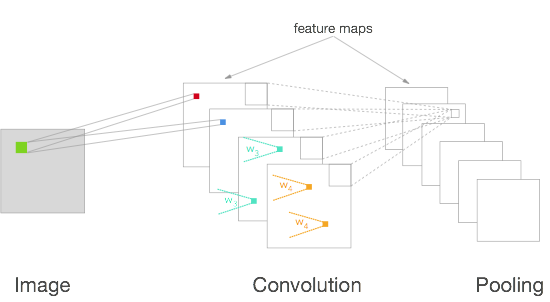
\includegraphics[width=0.6\textwidth]{figures/figures/convnet.png}
  \end{center}
  \caption[Example of a convolutional network architecture]{Example of a neural network architecture with convolutional and pooling layers.  Here, four separate convolutional filters are trained and pooled into a single feature map.  The structure can be repeated for several downstream feature maps.}
  \label{convnet}
\end{figure}

\subsection{Pooling}

With a large number of input pixels and many convolutional filters, the number of weights which must be learned can grow dramatically.
Pooling \cite{lecun2010convolutional} is a powerful technique for down-sample the number of parameters and thus reduce the complexity of the network.
In so-called \textit{max pooling}, down-sampling is achieved by taking the maximum value of each filter output in $n \times m$ sub-regions of the image.
An alternative to max pooling is \textit{average pooling}, where the average value is used instead of the maximum.  Pooling regions can be non-overlapping \cite{lecun2010convolutional}, or be allowed  to overlap \cite{szegedy2014going,krizhevsky2012imagenet}.
Pooling has also been used to combine the output of semantically similar feature maps by taking the maximum (or average) output over a group of feature maps\cite{lecun2015deep}.
Semantic similarity is imposed during training through the bottleneck of information flowing backwards through the pooling layers.  Layers which pool over feature maps are referred to as \textit{maxout} layers.

\subsection{Network-in-Network and \googlenet}

The Network-in-Network (NIN) \cite{lin2013network} approach has been used to augment the learning capacity of convolution layers while also reducing dimensionality.
Rather than using maxout feature pooling to reduce dimensionality, the NIN approach recombines features using a weighted sum of filter outputs with a \relu nonlinearity to produce a new set of features.
While NIN layers could be used with more output filters than input filters, they are more commonly used with fewer.
In that case, the NIN layers can be seen as synthesizing output across filters to produce a higher level, but more compact representation of the input filters.

\begin{figure}[t]
\begin{subfigure}[t]{0.5\textwidth}
                \centering
                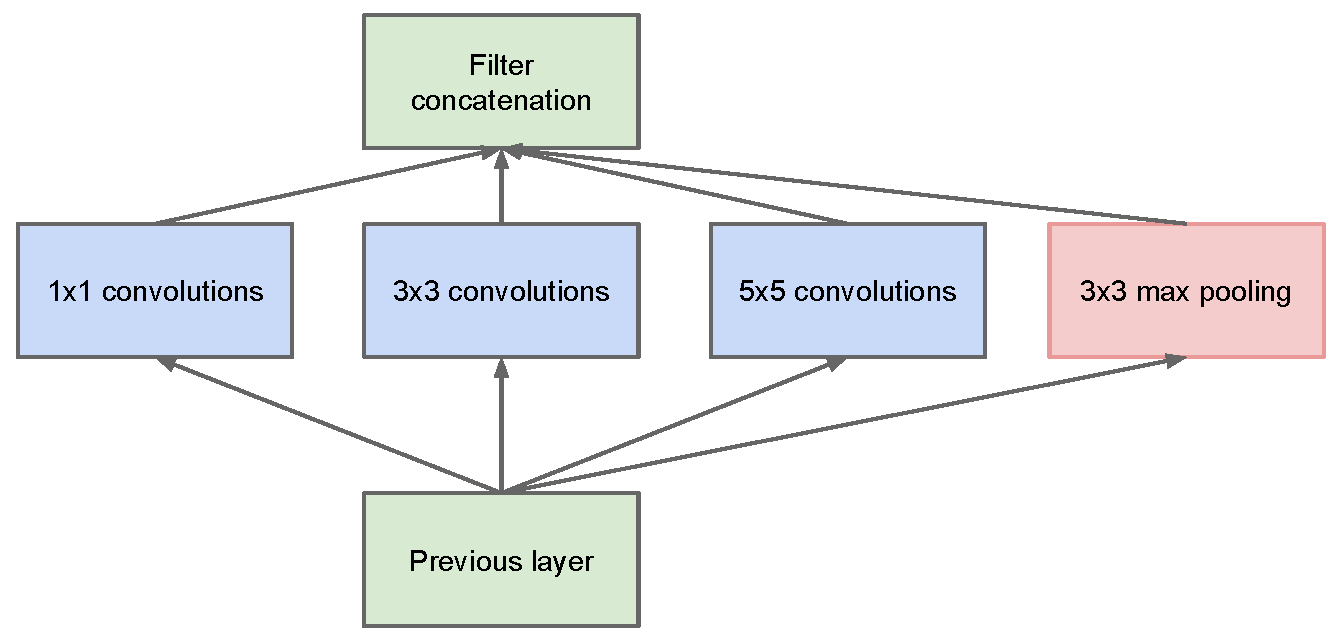
\includegraphics[width=0.9\textwidth]{figures/figures/inceptionnaive.pdf}
               \caption{Basic version of the inception module concept, which includes $1\times1$, $3\times3$, and $5\times5$ filters trained side-by-side.}
                 \label{basicinception}
        \end{subfigure}
        ~
\begin{subfigure}[t]{0.5\textwidth}
                \centering
                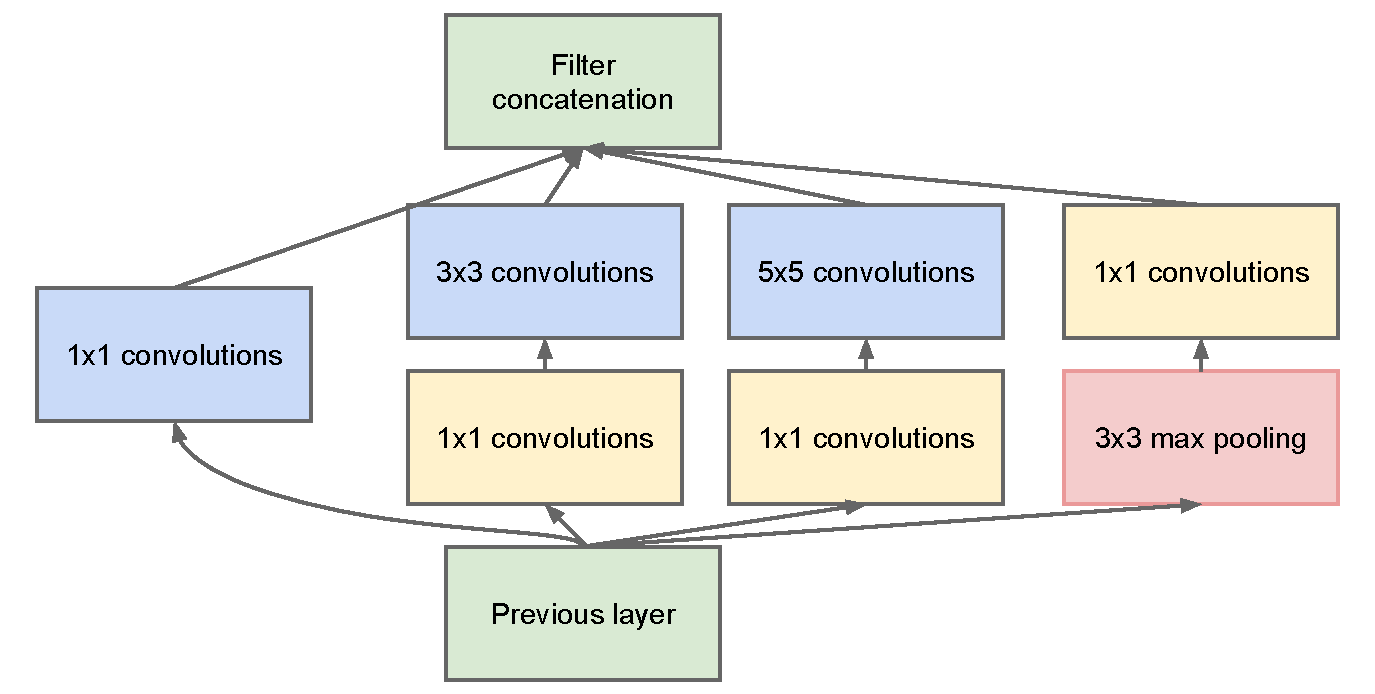
\includegraphics[width=0.9\textwidth]{figures/figures/inceptionmodule.pdf}
               \caption{Final design of exception module which uses $1\times1$ convolutions with NIN filter recombination to reduce dimensionality.}
                \label{fullinception}

        \end{subfigure}
        \caption{Inception module architecture.}
        \label{inception}
\end{figure}


The NIN approach has been used heavily in a leading network architecture known as \googlenet \cite{szegedy2014going}.
The \googlenet architecture is built up from a repeated structure dubbed the \textit{inception module}, as seen in figure \ref{inception}.
In the inception module, all $1\times1$ convolution layers are combined with a NIN recombination layer to reduce dimensionality.
Prior to more expensive $3\times3$ and $5\times5$ convolutions, the input filters are reduced down to 96 and 16 filters, respectively.
The $3\times3$ and $5\times5$ respectively include 128 and 32 filters, which are concatenated with the output of 64 $1\times1$ filters and another 32 $1\times1$ filters which follow $3\times3$ max pooling.  The full \googlenet, seen in figure \ref{googlenet} includes nine repetitions of the inception module.

Another important feature of \googlenet is the use of multiple softmax outputs to better train early layers \cite{szegedy2014going}.
\googlenet includes two extra outputs at upstream points in the network to propagate information backwards during training.
In the final classification result, these outputs are ignored, but during training they provide a less attenuated version of the error.
At any point in the network, the gradient used for training is the average of the gradient from each of the downstream softmax outputs.

\begin{figure}[t]
  \begin{center}
    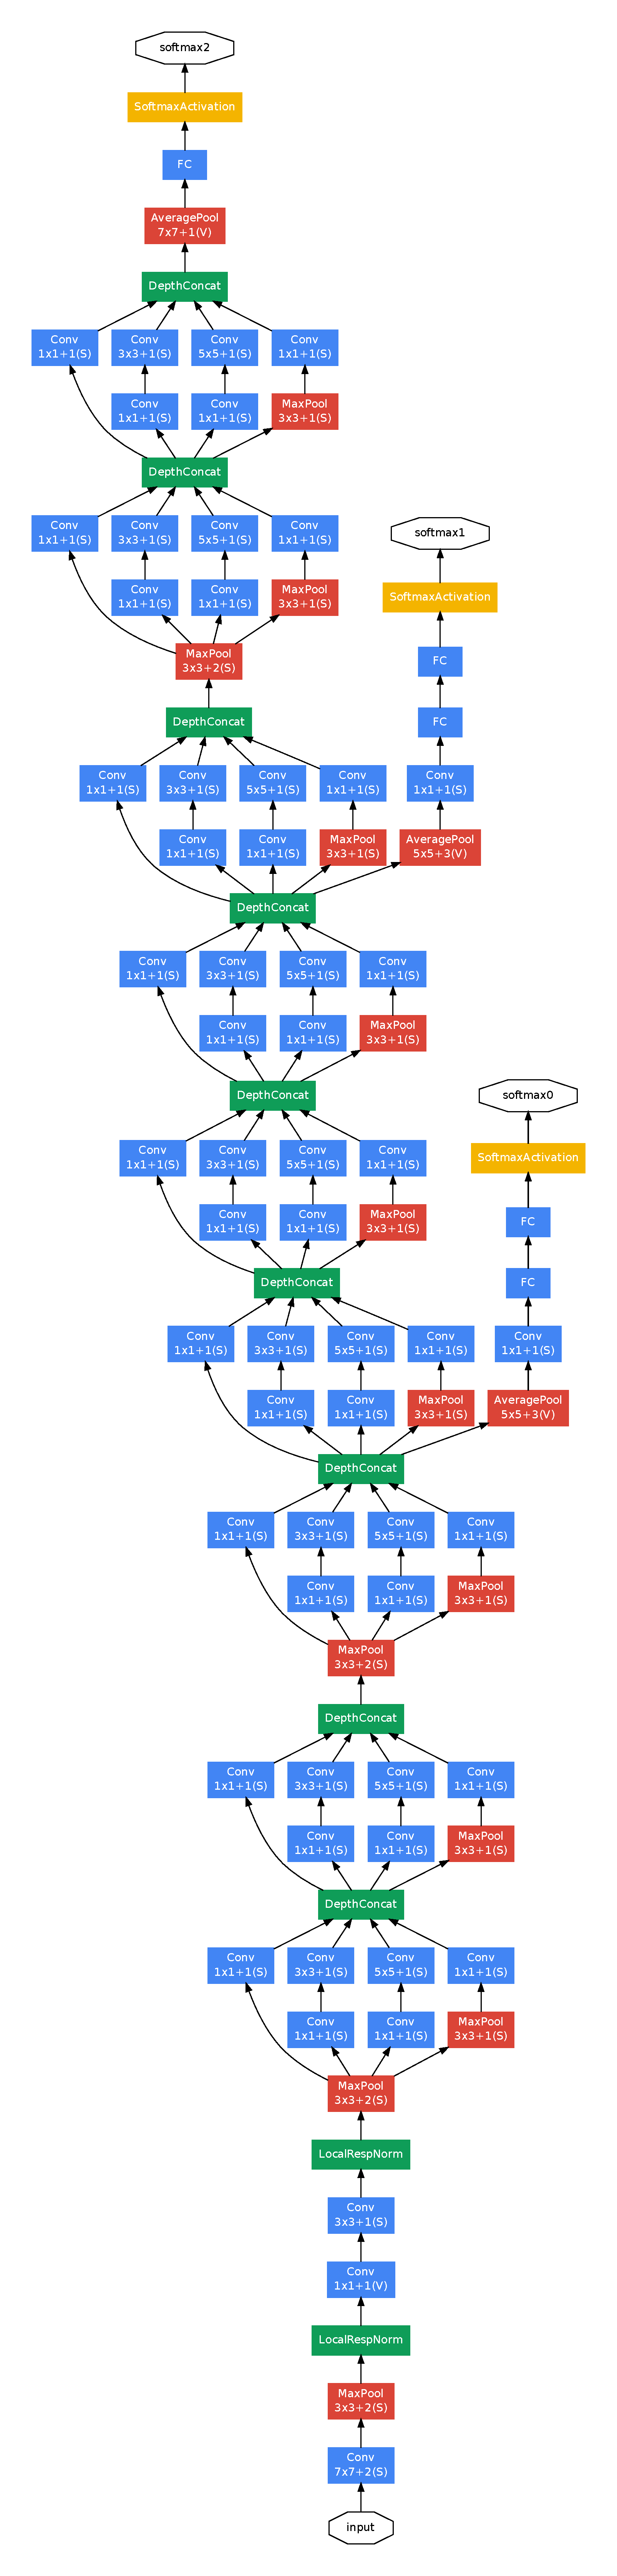
\includegraphics[height=\textheight]{figures/figures/inceptionoverall.pdf}
  \end{center}
  \caption[Complete \googlenet architecture]{Complete \googlenet archtecture, with 9 inception modules and upstream softmax outputs.}
  \label{googlenet}
\end{figure}

\subsection{Dropout Regularization}

Regularization refers to the prevention of overfitting during network training, that is, ensuring that the trained model generalized well beyond the training sample.
A common regularization technique is to include penalty terms in the cost function which proportional to the square or absolute value of the weights, thus constraining them them to remain small during training.
Keeping the weights small prevents the model from responding too strongly to any one input feature.

Recently, the technique of constraining weights has given way to a new technique called \textit{dropout} \cite{hinton2014dropout}.
Dropout a subset of of the weights in a layer to zero for a given training iteration.  On each iteration, each weight is set to zero with probability $r$, so a new different sample of weights is excluded at each iteration.
The inner product of the weights with the input, $z$ is scaled up by a factor of $1-r$ to roughly maintain the overall scale of the value passed through the nonlinearity.
Dropout with $r\approx 0.5$ proves to be a very robust regularizer and has quickly become the most popular technique used in the field \cite{lecun2015deep}.


%%%%%%%%%%%%%%%%%%%%%%%%%%%%%%%%%%%%%%%%%%%%%%%%%%%%%%%%%%%%%%%%%%%%%%%%%%%%%%%%
